\chapter{Introduction}
Computer vision applications on handheld devices have received growing interest in recent years. 
Modern smartphones are cheap, and their cameras and CPUs are good enough for many computer vision purposes.

Computer vision applications on smartphones have the potential to simplify many everyday tasks.
One such task is to measure the dimensions of an object.
This thesis investigates how the dimensions of cuboid packages can be measured from an image taken with the camera of a smartphone.

\section{Background}
In order to make measurements from an image, one must have some sense of the scale in the scene.
This can be achieved by placing an object of known size in the image, a \textit{reference object}.
The idea is that a common object, such as a credit card, is placed on top of the package.
If the positions of the reference object and the package are known in the image, it could be possible to calculate the dimensions of the package.

This process must essentially be automatic if this approach is to be an appealing alternative to measuring the package manually.
This fact places two important requirements on the application. Firstly, the reference object and the package must be detected automatically within the image. Secondly, the measuring procedure cannot require prior calibration.
%\begin{itemize}
%	\item The reference object and package must be detected automatically within the image.
%	\item The measuring procedure cannot require prior calibration.
%\end{itemize}

Computer vision applications which aim to extract metric information from a scene typically require knowledge about the internal properties of the camera.
A common way to gather this information is to perform a calibration procedure in advance, by observing a known calibration object, e.g. a printed paper with a special pattern on it.
In this scenario, a preparation step like this is very undesirable from a user perspective.
Therefore, gathering the necessary information can not require any additional steps, such as calibrating the camera manually.
In other words, the problem must be solved using an \textit{uncalibrated view}.

One way to determine the internal properties of the camera without manual calibration is to use the geometry in the image to calibrate.
More specifically, the \textit{vanishing points} in the image can be used to calibrate the camera.
Vanishing points are points where lines which are parallel in the world (but not in the image) meet.
It can be shown that three orthogonal vanishing points are enough to calibrate a camera from a single image \cite[p. 226]{hartley-zisserman}.

Vanishing point calibration can be problematic in general, since every image does not have vanishing points, let alone three orthogonal ones.
Additionally, they can be difficult to find even when present.
In this case however, it is ideal, since every cuboid gives rise to three orthogonal vanishing points, as seen in figure \ref{fig:vanishing_points}.

\begin{figure}
\begin{center}
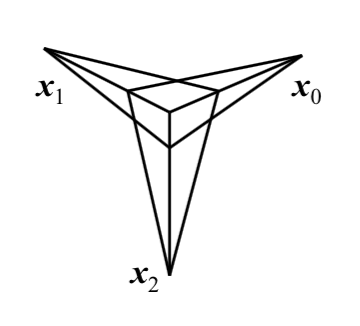
\includegraphics[width=0.6\textwidth]{figures/vanishing_points.png}
\end{center}
\credit{\cite[p. 330]{szeliski}}
\caption[Vanishing points induced by the edges of a cuboid]{Visualisation of how the edges of a cuboid give rise to three orthogonal vanishing points: $x_0$, $x_1$, and $x_2$.}
\label{fig:vanishing_points}
\end{figure}

%\section{Requirements} \label{introduction:requirements} TODO fix label


%A measuring application must not only be easy to use, it must also have good performance.
%Performance can be broken down to three key aspects: robustness, accuracy and speed.
%Robustness is defined as the success rate of the method, i.e. the rate at which an adequately correct result is achieved.
%Accuracy is defined as the average precision of the result when a correct result is achieved.
%Speed refers to the average processing time.
%
%The ultimate goal with regard to speed is to reach real time performance, i.e. processing times of less than 30-40 milliseconds per frame \cite{pulli2012real}.
%This is a challenging goal, especially with the limited processing power of a mobile device.
%However, in this case it is considered more important that the method is accurate and robust, short processing times are a secondary goal.
%Still, as a step to reduce processing time, and to reduce the computational complexity of the method, only a single image will be used at a time, as opposed to analysing multiple images and before delivering an answer.
%In other words, the problem will be solved using a \textit{single uncalibrated view}.

\section{Problem statement}\label{problem-statement}
This thesis investigates the automatic detection and measuring of cuboid packages from uncalibrated views.

%The goal of this thesis is to implement and evaluate a method to automatically measure the dimensions of cuboid packages with a mobile device, using a single uncalibrated view.
This will be done by placing a known reference object on top of the package, and taking pictures of the package and reference object together.
The package and reference object will be detected and localised automatically by the application, after which the dimensions of the package will be calculated.

A model-based approach will be used for detection, since it should be easy to create a model to detect cuboids, due to their well-defined shape.
%The detector will use the edge information in the image to model the package.

Uncalibrated measurements will be achieved by using the vanishing points formed by the edges of the package to determine the internal parameters of the camera.	
It is clear from \cite{hartley-zisserman} that it is possible to calibrate the camera from three orthogonal vanishing points (if some assumptions are made about the camera), but it is unclear if the result is accurate enough to make good measurements, especially when the error of detection is factored in. 
As presented further in section \ref{related_work:vanishing_point_calibration} the related work uses either multiple views or a large amount of lines in the image to find the vanishing points.
Here, maximum three lines will contribute to each vanishing point in a single image, which may reduce accuracy.

In order to reduce complexity, it is desirable to constrain the solution to use a \textit{single} view to measure the package.
It is not obvious that it is possible even once the internal parameters and the positions of the package and the reference object are known.
It is certainly not possible to make arbitrary measurements in a single image using this information, but it could be made possible to measure the package by once again using its cuboid shape.

To summarise, this thesis aims to answer the following questions:
\begin{itemize}
	\item How well can cuboid packages be detected with a model-based detector?
	\item How well can measurements be made when calibration is done using three orthogonal vanishing points in a single image?
	\item Is it possible to measure cuboid packages from a single view?
\end{itemize}

\section{Purpose}
The purpose of this thesis is to determine the feasibility of automatically measuring cuboid packages on a handheld device.
This will be done by using existing methods and applying them in a new way.
For example, it is not common to both calibrate the camera and make measurements from the same, single image.

This specific setting also provides interesting challenges.
The application must have high success rate and accuracy in order to be useful.
It must also be fast, since handheld devices have limited processing power and users have limited patience.

\section{Method}
It is clear that this approach requires two components: a detection component and a measuring component.
The detection component should find the positions of the reference object and the package in the image, and the measuring component should use their positions to calculate the dimensions of the package.
Both are equally important for the performance of the full system.

To asses the quality of the system, the two components will be evaluated both in isolation and combined.
The evaluation will test success rate and accuracy.
Success rate is defined as the rate at which the result is reasonably correct.
Accuracy refers to the average accuracy based on the successful results.

As stated earlier, using uncalibrated views was a requirement for the sake of convenience.
However, while using an uncalibrated view is more convenient, a calibrated view is expected to yield higher accuracy.
If so, it would be interesting to know how much accuracy needs to be sacrificed to gain the extra utility of not needing prior calibration.
In order to determine this, a version which uses a calibrated view will also be implemented.
The calibrated version will serve as a baseline implementation, to which the performance of the uncalibrated method will be compared.

In principle, all of the above can be tested offline, using pictures taken with a smartphone.
This will be the primary method used when evaluating the result.
However, since the purpose of the program is to be used in a smartphone, it will also be embedded in a demo application for a smartphone, to assert that it performs well enough in its intended environment and that the program is fast enough to be used in a smartphone.

\section{Delimitations} \label{introduction:delimitations}
In a finished consumer application, it would be desirable to have the option to choose between a multitude of reference objects, like credit cards, matchboxes, smartphones, papers, and more. 
To simplify the detection component, only white papers from the ISO 216 A-series (e.g. A4 or A5) will be considered as reference objects in this thesis.
The reason behind this choice is that papers of this type are very common, and should be easy to detect.

The type of packages considered are limited to packages with a cuboid shape, and with a colour that has reasonable contrast to that of the reference object.
Furthermore only untextured, or lightly textured packages are considered.

The package is assumed to be placed on a flat surface.
It is also assumed to not be occluded, and the scene is assumed to not contain much clutter.